\documentclass[12pt]{book}

\usepackage{xeCJK}
\usepackage{listings}
\usepackage{multirow}
\usepackage{longtable}
\usepackage{fontspec}
\usepackage{ctex}
\usepackage[top=3cm,bottom=3cm,left=3cm,right=3cm, headsep=10pt,a4paper]{geometry} % Page margins
\usepackage{graphicx} % Required for including pictures
\graphicspath{{Pictures/}{Image/common/}} % Specifies the directory where pictures are stored
\usepackage{lipsum} % Inserts dummy text
\usepackage[ddmmyyyy]{datetime}
\usepackage{tikz} % Required for drawing custom shapes
\usepackage[english]{babel} % English language/hyphenation
\usepackage{enumitem} % Customize lists
\setlist{nolistsep} % Reduce spacing between bullet points and numbered lists
\usepackage{booktabs} % Required for nicer horizontal rules in tables
\usepackage{xcolor} % Required for specifying colors by name
\definecolor{ocre}{RGB}{243,102,25} % Define the orange color used for highlighting throughout the book
\usepackage{avant} % Use the Avantgarde font for headings
%\usepackage{times} % Use the Times font for headings
\usepackage{mathptmx} % Use the Adobe Times Roman as the default text font together with math symbols from the Sym­bol, Chancery and Com­puter Modern fonts
\usepackage{microtype} % Slightly tweak font spacing for aesthetics
\usepackage[T1]{fontenc}
\usepackage[utf8]{inputenc}
{\renewcommand{\bibname}{References}}
\usepackage[backend=bibtex,style=numeric]{biblatex}

\defbibheading{bibempty}{}

\usepackage{calc} % 简单的计算功能
\usepackage{makeidx} % 创建索引
\makeindex % Tells LaTeX to create the files required for indexing
\usepackage{titletoc} % 目录操作
\usepackage[bookmarksopen,bookmarksdepth=3]{hyperref}


%When compile under liunx% 

%\setCJKmainfont{WenQuanYi Micro Hei} % 设置缺省中文字体

\contentsmargin{0cm} % Removes the default margin

\lstdefinelanguage{JavaScript}{
	keywords={typeof, new, true, false, catch, function, return, null, catch, switch, var, if, in, while, do, else, case, break},
	keywordstyle=\color{blue}\bfseries,
	ndkeywords={class, export, boolean, throw, implements, import, this},
	ndkeywordstyle=\color{darkgray}\bfseries,
	identifierstyle=\color{black},
	sensitive=false,
	comment=[l]{//},
	morecomment=[s]{/*}{*/},
	commentstyle=\color{purple}\ttfamily,
	stringstyle=\color{red}\ttfamily,
	morestring=[b]',
	morestring=[b]"
}

%Figure显示为中文的“图”
\renewcommand\figurename{图}

\setcounter{tocdepth}{2}

%Set Code Format%
\lstloadlanguages{C, csh, make,python,Java,JavaScript}
\lstset{	  
	alsolanguage= XML,  
	tabsize=4, %  
	frame=shadowbox, %把代码用带有阴影的框圈起来  
	commentstyle=\color{red!50!green!50!blue!50},%浅灰色的注释
	frameround=tttt,  
	rulesepcolor=\color{red!20!green!20!blue!20},%代码块边框为淡青色  
	keywordstyle=\color{blue!90}\bfseries, %代码关键字的颜色为蓝色,粗体  
	showstringspaces=false,%不显示代码字符串中间的空格标记  
	stringstyle=\ttfamily, % 代码字符串的特殊格式  
	keepspaces=true, %  
	breakindent=22pt, % 
	breaklines=true,%设置代码自动换行 
	numbers=left,%左侧显示行号 往左靠,还可以为right,或none,即不加行号  
	stepnumber=1,%若设置为2,则显示行号为1,3,5,即stepnumber为公差,默认stepnumber=1  
	%numberstyle=\tiny, %行号字体用小号  
	numberstyle={\color[RGB]{0,192,192}\tiny},%设置行号的大小,大小有tiny,scriptsize,footnotesize,small,normalsize,large等  
	numbersep=8pt,  %设置行号与代码的距离,默认是5pt  
	basicstyle=\ttfamily, % 这句设置代码的大小  
	showspaces=false, % 
	escapechar=`,
	flexiblecolumns=true, %  
	breaklines=true, %对过长的代码自动换行  
	breakautoindent=true,%  
	breakindent=4em, %  	   
	aboveskip=1em, %代码块边框  
	tabsize=4,  
	showstringspaces=false, %不显示字符串中的空格  
	backgroundcolor=\color[RGB]{245,245,244},   %代码背景色  
	%backgroundcolor=\color[rgb]{0.91,0.91,0.91}    %添加背景色  
	escapeinside={``}{\_},  %在``里显示中文  
	%% added by http://bbs.ctex.org/viewthread.php?tid=53451  
	fontadjust,  
	captionpos=t,  
	framextopmargin=2pt,
	framexbottommargin=2pt,
	abovecaptionskip=-3pt,
	belowcaptionskip=3pt,  
	xleftmargin=4em,
	xrightmargin=4em, % 设定listing左右的空白  
	texcl=true
}

% Part text styling
\titlecontents{part}[0cm]{\addvspace{20pt}\centering\large\sffamily}{}{}{}

% Chapter text styling
\titlecontents{chapter}[1.25cm] % Indentation
{\addvspace{12pt}\large\sffamily\bfseries} % Spacing and font options for chapters
{\color{ocre!60}\contentslabel[\Large\thecontentslabel]{1.25cm}\color{ocre}} % Chapter number
{\color{ocre}}  
{\color{ocre!60}\normalsize\;\titlerule*[.5pc]{.}\;\thecontentspage} % Page number

% Section text styling
\titlecontents{section}[1.25cm] % Indentation
{\addvspace{3pt}\sffamily\bfseries} % Spacing and font options for sections
{\contentslabel[\thecontentslabel]{1.25cm}} % Section number
{}
{\hfill\color{black}\thecontentspage} % Page number
[]

% Subsection text styling
\titlecontents{subsection}[1.25cm] % Indentation
{\addvspace{1pt}\sffamily\small} % Spacing and font options for subsections
{\contentslabel[\thecontentslabel]{1.25cm}} % Subsection number
{}
{\ \titlerule*[.5pc]{.}\;\thecontentspage} % Page number
[]

% List of figures
\titlecontents{figure}[0em]
{\addvspace{-5pt}\sffamily}
{\thecontentslabel\hspace*{1em}}
{}
{\ \titlerule*[.5pc]{.}\;\thecontentspage}
[]

% List of tables
\titlecontents{table}[0em]
{\addvspace{-5pt}\sffamily}
{\thecontentslabel\hspace*{1em}}
{}
{\ \titlerule*[.5pc]{.}\;\thecontentspage}
[]

%----------------------------------------------------------------------------------------
%	MINI TABLE OF CONTENTS IN PART HEADS
%----------------------------------------------------------------------------------------

% Chapter text styling
\titlecontents{lchapter}[0em] % Indenting
{\addvspace{15pt}\large\sffamily\bfseries} % Spacing and font options for chapters
{\color{ocre}\contentslabel[\Large\thecontentslabel]{1.25cm}\color{ocre}} % Chapter number
{}  
{\color{ocre}\normalsize\sffamily\bfseries\;\titlerule*[.5pc]{.}\;\thecontentspage} % Page number

% Section text styling
\titlecontents{lsection}[0em] % Indenting
{\sffamily\small} % Spacing and font options for sections
{\contentslabel[\thecontentslabel]{1.25cm}} % Section number
{}
{}

% Subsection text styling
\titlecontents{lsubsection}[.5em] % Indentation
{\normalfont\footnotesize\sffamily} % Font settings
{}
{}
{}

%----------------------------------------------------------------------------------------
%	PAGE HEADERS
%----------------------------------------------------------------------------------------

\usepackage{fancyhdr} % Required for header and footer configuration

\pagestyle{fancy}
\renewcommand{\chaptermark}[1]{\markboth{\sffamily\normalsize\bfseries\chaptername\ \thechapter.\ #1}{}} % Chapter text font settings
\renewcommand{\sectionmark}[1]{\markright{\sffamily\normalsize\thesection\hspace{5pt}#1}{}} % Section text font settings
\fancyhf{} \fancyhead[LE,RO]{\sffamily\normalsize\thepage} % Font setting for the page number in the header
\fancyhead[LO]{\rightmark} % Print the nearest section name on the left side of odd pages
\fancyhead[RE]{\leftmark} % Print the current chapter name on the right side of even pages
\renewcommand{\headrulewidth}{0.5pt} % Width of the rule under the header
\addtolength{\headheight}{2.5pt} % Increase the spacing around the header slightly
\renewcommand{\footrulewidth}{0pt} % Removes the rule in the footer
\fancypagestyle{plain}{\fancyhead{}\renewcommand{\headrulewidth}{0pt}} % Style for when a plain pagestyle is specified

% Removes the header from odd empty pages at the end of chapters
\makeatletter
\renewcommand{\cleardoublepage}{
	\clearpage\ifodd\c@page\else
	\hbox{}
	\vspace*{\fill}
	\thispagestyle{empty}
	\newpage
	\fi}

%----------------------------------------------------------------------------------------
%	THEOREM STYLES
%----------------------------------------------------------------------------------------

\usepackage{amsmath,amsfonts,amssymb,amsthm} % For math equations, theorems, symbols, etc

\newcommand{\intoo}[2]{\mathopen{]}#1\,;#2\mathclose{[}}
\newcommand{\ud}{\mathop{\mathrm{{}d}}\mathopen{}}
\newcommand{\intff}[2]{\mathopen{[}#1\,;#2\mathclose{]}}
\newtheorem{notation}{Notation}[chapter]

% Boxed/framed environments
\newtheoremstyle{ocrenumbox}% % Theorem style name
{0pt}% Space above
{0pt}% Space below
{\normalfont}% % Body font
{}% Indent amount
{\small\bf\sffamily\color{ocre}}% % Theorem head font
{\;}% Punctuation after theorem head
{0.25em}% Space after theorem head
{\small\sffamily\color{ocre}\thmname{#1}\nobreakspace\thmnumber{\@ifnotempty{#1}{}\@upn{#2}}% Theorem text (e.g. Theorem 2.1)
	\thmnote{\nobreakspace\the\thm@notefont\sffamily\bfseries\color{black}---\nobreakspace#3.}} % Optional theorem note
\renewcommand{\qedsymbol}{$\blacksquare$}% Optional qed square

\newtheoremstyle{blacknumex}% Theorem style name
{5pt}% Space above
{5pt}% Space below
{\normalfont}% Body font
{} % Indent amount
{\small\bf\sffamily}% Theorem head font
{\;}% Punctuation after theorem head
{0.25em}% Space after theorem head
{\small\sffamily{\tiny\ensuremath{\blacksquare}}\nobreakspace\thmname{#1}\nobreakspace\thmnumber{\@ifnotempty{#1}{}\@upn{#2}}% Theorem text (e.g. Theorem 2.1)
	\thmnote{\nobreakspace\the\thm@notefont\sffamily\bfseries---\nobreakspace#3.}}% Optional theorem note

\newtheoremstyle{blacknumbox} % Theorem style name
{0pt}% Space above
{0pt}% Space below
{\normalfont}% Body font
{}% Indent amount
{\small\bf\sffamily}% Theorem head font
{\;}% Punctuation after theorem head
{0.25em}% Space after theorem head
{\small\sffamily\thmname{#1}\nobreakspace\thmnumber{\@ifnotempty{#1}{}\@upn{#2}}% Theorem text (e.g. Theorem 2.1)
	\thmnote{\nobreakspace\the\thm@notefont\sffamily\bfseries---\nobreakspace#3.}}% Optional theorem note

% Non-boxed/non-framed environments
\newtheoremstyle{ocrenum}% % Theorem style name
{5pt}% Space above
{5pt}% Space below
{\normalfont}% % Body font
{}% Indent amount
{\small\bf\sffamily\color{ocre}}% % Theorem head font
{\;}% Punctuation after theorem head
{0.25em}% Space after theorem head
{\small\sffamily\color{ocre}\thmname{#1}\nobreakspace\thmnumber{\@ifnotempty{#1}{}\@upn{#2}}% Theorem text (e.g. Theorem 2.1)
	\thmnote{\nobreakspace\the\thm@notefont\sffamily\bfseries\color{black}---\nobreakspace#3.}} % Optional theorem note
\renewcommand{\qedsymbol}{$\blacksquare$}% Optional qed square
\makeatother 

% Defines the theorem text style for each type of theorem to one of the three styles above
\newcounter{dummy} 
\numberwithin{dummy}{section}
\theoremstyle{ocrenumbox}
\newtheorem{theoremeT}[dummy]{Theorem}
\newtheorem{problem}{Problem}[chapter]
\newtheorem{exerciseT}{Exercise}[chapter]
\theoremstyle{blacknumex}
\newtheorem{exampleT}{Example}[chapter]
\theoremstyle{blacknumbox}
\newtheorem{vocabulary}{Vocabulary}[chapter]
\newtheorem{definitionT}{Definition}[section]
\newtheorem{corollaryT}[dummy]{Corollary}
\theoremstyle{ocrenum}
\newtheorem{proposition}[dummy]{Proposition}

%----------------------------------------------------------------------------------------
%	DEFINITION OF COLORED BOXES
%----------------------------------------------------------------------------------------

\RequirePackage[framemethod=default]{mdframed} % Required for creating the theorem, definition, exercise and corollary boxes

% Theorem box
\newmdenv[skipabove=7pt,
skipbelow=7pt,
backgroundcolor=black!5,
linecolor=ocre,
innerleftmargin=5pt,
innerrightmargin=5pt,
innertopmargin=5pt,
leftmargin=0cm,
rightmargin=0cm,
innerbottommargin=5pt]{tBox}

% Exercise box	  
\newmdenv[skipabove=7pt,
skipbelow=7pt,
rightline=false,
leftline=true,
topline=false,
bottomline=false,
backgroundcolor=ocre!10,
linecolor=ocre,
innerleftmargin=5pt,
innerrightmargin=5pt,
innertopmargin=5pt,
innerbottommargin=5pt,
leftmargin=0cm,
rightmargin=0cm,
linewidth=4pt]{eBox}	

% Definition box
\newmdenv[skipabove=7pt,
skipbelow=7pt,
rightline=false,
leftline=true,
topline=false,
bottomline=false,
linecolor=ocre,
innerleftmargin=5pt,
innerrightmargin=5pt,
innertopmargin=0pt,
leftmargin=0cm,
rightmargin=0cm,
linewidth=4pt,
innerbottommargin=0pt]{dBox}	

% Corollary box
\newmdenv[skipabove=7pt,
skipbelow=7pt,
rightline=false,
leftline=true,
topline=false,
bottomline=false,
linecolor=gray,
backgroundcolor=black!5,
innerleftmargin=5pt,
innerrightmargin=5pt,
innertopmargin=5pt,
leftmargin=0cm,
rightmargin=0cm,
linewidth=4pt,
innerbottommargin=5pt]{cBox}

% Creates an environment for each type of theorem and assigns it a theorem text style from the "Theorem Styles" section above and a colored box from above
\newenvironment{theorem}{\begin{tBox}\begin{theoremeT}}{\end{theoremeT}\end{tBox}}
\newenvironment{exercise}{\begin{eBox}\begin{exerciseT}}{\hfill{\color{ocre}\tiny\ensuremath{\blacksquare}}\end{exerciseT}\end{eBox}}				  
\newenvironment{definition}{\begin{dBox}\begin{definitionT}}{\end{definitionT}\end{dBox}}	
\newenvironment{example}{\begin{exampleT}}{\hfill{\tiny\ensuremath{\blacksquare}}\end{exampleT}}		
\newenvironment{corollary}{\begin{cBox}\begin{corollaryT}}{\end{corollaryT}\end{cBox}}	

%----------------------------------------------------------------------------------------
%	REMARK ENVIRONMENT
%----------------------------------------------------------------------------------------

\newenvironment{remark}{\par\vspace{10pt}\small % Vertical white space above the remark and smaller font size
	\begin{list}{}{
			\leftmargin=35pt % Indentation on the left
			\rightmargin=25pt}\item\ignorespaces % Indentation on the right
		\makebox[-2.5pt]{\begin{tikzpicture}[overlay]
			\node[draw=ocre!60,line width=1pt,circle,fill=ocre!25,font=\sffamily\bfseries,inner sep=2pt,outer sep=0pt] at (-15pt,0pt){\textcolor{ocre}{R}};\end{tikzpicture}} % Orange R in a circle
		\advance\baselineskip -1pt}{\end{list}\vskip5pt} % Tighter line spacing and white space after remark

%----------------------------------------------------------------------------------------
%	SECTION NUMBERING IN THE MARGIN
%----------------------------------------------------------------------------------------

\makeatletter
\renewcommand{\@seccntformat}[1]{\llap{\textcolor{ocre}{\csname the#1\endcsname}\hspace{1em}}}                    
\renewcommand{\section}{\@startsection{section}{1}{\z@}
	{-4ex \@plus -1ex \@minus -.4ex}
	{1ex \@plus.2ex }
	{\normalfont\large\sffamily\bfseries}}
\renewcommand{\subsection}{\@startsection {subsection}{2}{\z@}
	{-3ex \@plus -0.1ex \@minus -.4ex}
	{0.5ex \@plus.2ex }
	{\normalfont\sffamily\bfseries}}
\renewcommand{\subsubsection}{\@startsection {subsubsection}{3}{\z@}
	{-2ex \@plus -0.1ex \@minus -.2ex}
	{.2ex \@plus.2ex }
	{\normalfont\small\sffamily\bfseries}}                        
\renewcommand\paragraph{\@startsection{paragraph}{4}{\z@}
	{-2ex \@plus-.2ex \@minus .2ex}
	{.1ex}
	{\normalfont\small\sffamily\bfseries}}

%----------------------------------------------------------------------------------------
%	PART HEADINGS
%----------------------------------------------------------------------------------------

% numbered part in the table of contents
\newcommand{\@mypartnumtocformat}[2]{%
	\setlength\fboxsep{0pt}%
	\noindent\colorbox{ocre!20}{\strut\parbox[c][.7cm]{\ecart}{\color{ocre!70}\Large\sffamily\bfseries\centering#1}}\hskip\esp\colorbox{ocre!40}{\strut\parbox[c][.7cm]{\linewidth-\ecart-\esp}{\Large\sffamily\centering#2}}}%
%%%%%%%%%%%%%%%%%%%%%%%%%%%%%%%%%%
% unnumbered part in the table of contents
\newcommand{\@myparttocformat}[1]{%
	\setlength\fboxsep{0pt}%
	\noindent\colorbox{ocre!40}{\strut\parbox[c][.7cm]{\linewidth}{\Large\sffamily\centering#1}}}%
%%%%%%%%%%%%%%%%%%%%%%%%%%%%%%%%%%
\newlength\esp
\setlength\esp{4pt}
\newlength\ecart
\setlength\ecart{1.2cm-\esp}
\newcommand{\thepartimage}{}%
\newcommand{\partimage}[1]{\renewcommand{\thepartimage}{#1}}%
\def\@part[#1]#2{%
	\ifnum \c@secnumdepth >-2\relax%
	\refstepcounter{part}%
	\addcontentsline{toc}{part}{\texorpdfstring{\protect\@mypartnumtocformat{\thepart}{#1}}{\partname~\thepart\ ---\ #1}}
	\else%
	\addcontentsline{toc}{part}{\texorpdfstring{\protect\@myparttocformat{#1}}{#1}}%
	\fi%
	\startcontents%
	\markboth{}{}%
	{\thispagestyle{empty}%
		\begin{tikzpicture}[remember picture,overlay]%
		\node at (current page.north west){\begin{tikzpicture}[remember picture,overlay]%	
			\fill[ocre!20](0cm,0cm) rectangle (\paperwidth,-\paperheight);
			\node[anchor=north] at (4cm,-3.25cm){\color{ocre!40}\fontsize{220}{100}\sffamily\bfseries\@Roman\c@part}; 
			\node[anchor=south east] at (\paperwidth-1cm,-\paperheight+1cm){\parbox[t][][t]{8.5cm}{
					\printcontents{l}{0}{\setcounter{tocdepth}{1}}%
			}};
			\node[anchor=north east] at (\paperwidth-1.5cm,-3.25cm){\parbox[t][][t]{15cm}{\strut\raggedleft\color{white}\fontsize{30}{30}\sffamily\bfseries#2}};
			\end{tikzpicture}};
\end{tikzpicture}}%
\@endpart}
\def\@spart#1{%
\startcontents%
\phantomsection
{\thispagestyle{empty}%
	\begin{tikzpicture}[remember picture,overlay]%
	\node at (current page.north west){\begin{tikzpicture}[remember picture,overlay]%	
		\fill[ocre!20](0cm,0cm) rectangle (\paperwidth,-\paperheight);
		\node[anchor=north east] at (\paperwidth-1.5cm,-3.25cm){\parbox[t][][t]{15cm}{\strut\raggedleft\color{white}\fontsize{30}{30}\sffamily\bfseries#1}};
		\end{tikzpicture}};
\end{tikzpicture}}
\addcontentsline{toc}{part}{\texorpdfstring{%
	\setlength\fboxsep{0pt}%
	\noindent\protect\colorbox{ocre!40}{\strut\protect\parbox[c][.7cm]{\linewidth}{\Large\sffamily\protect\centering #1\quad\mbox{}}}}{#1}}%
\@endpart}
\def\@endpart{\vfil\newpage
\if@twoside
\if@openright
\null
\thispagestyle{empty}%
\newpage
\fi
\fi
\if@tempswa
\twocolumn
\fi}

%----------------------------------------------------------------------------------------
%	CHAPTER HEADINGS
%----------------------------------------------------------------------------------------

% A switch to conditionally include a picture, implemented by  Christian Hupfer
\newif\ifusechapterimage
\usechapterimagetrue
\newcommand{\thechapterimage}{}%
\newcommand{\chapterimage}[1]{\ifusechapterimage\renewcommand{\thechapterimage}{#1}\fi}%
\def\@makechapterhead#1{%
{\parindent \z@ \raggedright \normalfont
\ifnum \c@secnumdepth >\m@ne
\if@mainmatter
\begin{tikzpicture}[remember picture,overlay]
\node at (current page.north west)
{\begin{tikzpicture}[remember picture,overlay]
	\node[anchor=north west,inner sep=0pt] at (0,0) {\ifusechapterimage\includegraphics[width=\paperwidth]{\thechapterimage}\fi};
	\draw[anchor=west] (\Gm@lmargin,-9cm) node [line width=2pt,rounded corners=15pt,draw=ocre,fill=white,fill opacity=0.5,inner sep=15pt]{\strut\makebox[22cm]{}};
	\draw[anchor=west] (\Gm@lmargin+.3cm,-9cm) node {\huge\sffamily\bfseries\color{black}\thechapter. #1\strut};
	\end{tikzpicture}};
\end{tikzpicture}
\else
\begin{tikzpicture}[remember picture,overlay]
\node at (current page.north west)
{\begin{tikzpicture}[remember picture,overlay]
\node[anchor=north west,inner sep=0pt] at (0,0) {\ifusechapterimage\includegraphics[width=\paperwidth]{\thechapterimage}\fi};
\draw[anchor=west] (\Gm@lmargin,-9cm) node [line width=2pt,rounded corners=15pt,draw=ocre,fill=white,fill opacity=0.5,inner sep=15pt]{\strut\makebox[22cm]{}};
\draw[anchor=west] (\Gm@lmargin+.3cm,-9cm) node {\huge\sffamily\bfseries\color{black}#1\strut};
\end{tikzpicture}};
\end{tikzpicture}
\fi\fi\par\vspace*{270\p@}}}

%-------------------------------------------

\def\@makeschapterhead#1{%
\begin{tikzpicture}[remember picture,overlay]
\node at (current page.north west)
{\begin{tikzpicture}[remember picture,overlay]
\node[anchor=north west,inner sep=0pt] at (0,0) {\ifusechapterimage\includegraphics[width=\paperwidth]{\thechapterimage}\fi};
\draw[anchor=west] (\Gm@lmargin,-9cm) node [line width=2pt,rounded corners=15pt,draw=ocre,fill=white,fill opacity=0.5,inner sep=15pt]{\strut\makebox[22cm]{}};
\draw[anchor=west] (\Gm@lmargin+.3cm,-9cm) node {\huge\sffamily\bfseries\color{black}#1\strut};
\end{tikzpicture}};
\end{tikzpicture}
\par\vspace*{270\p@}}
\makeatother

%----------------------------------------------------------------------------------------
%	HYPERLINKS IN THE DOCUMENTS
%----------------------------------------------------------------------------------------

\usepackage{hyperref}
\hypersetup{hidelinks,backref=true,pagebackref=true,hyperindex=true,colorlinks=false,breaklinks=true,urlcolor= ocre,bookmarks=true,bookmarksopen=false,pdftitle={Title},pdfauthor={Author}}
\usepackage{bookmark}
\bookmarksetup{
open,
numbered,
addtohook={%
\ifnum\bookmarkget{level}=0 % chapter
\bookmarksetup{bold}%
\fi
\ifnum\bookmarkget{level}=-1 % part
\bookmarksetup{color=ocre,bold}%
\fi
}
}

\addbibresource{Bronvermelding.bib} 

\begin{document}

\begingroup
\thispagestyle{empty}
\begin{tikzpicture}[remember picture,overlay]
\coordinate [below=12cm] (midpoint) at (current page.north);
\node at (current page.north west)
{\begin{tikzpicture}[remember picture,overlay]
\node[anchor=north west,inner sep=0pt] at (0,0) {
\includegraphics[width=\paperwidth]{background}}; % Background image
\draw[anchor=north] (midpoint) node [fill=ocre!30!white,fill opacity=0.6,text opacity=1,inner sep=1cm]{\Huge\centering\bfseries\sffamily\parbox[c][][t]{\paperwidth}{\centering 开发记录 \\[15pt] % Book title
{\Large 卷一}\\[20pt] % Subtitle
{\large Dolphin}}}; % Author name
\end{tikzpicture}};
\end{tikzpicture}
\vfill
\endgroup


%----------------------------------------------------------------------------------------
%	BLANK PAGE
%----------------------------------------------------------------------------------------

\newpage
~\vfill
\thispagestyle{empty}

%----------------------------------------------------------------------------------------
%	COPYRIGHT PAGE
%----------------------------------------------------------------------------------------

\newpage
~\vfill
\thispagestyle{empty}

\noindent Copyright \textcopyright\ 2017 Xiaoqiang Jiang\\ % Copyright notice

\noindent \textsc{Edited by Xiaoqiang Jiang}\\ % Publisher

\noindent \textsc{\url{http://jiangxiaoqiang.github.com/}}\\

\noindent All Rights Reserved.\\ % License information

\noindent \textit{Version \currenttime, \today} % Printing/edition date


%----------------------------------------------------------------------------------------
%	TABLE OF CONTENTS
%----------------------------------------------------------------------------------------

%\usechapterimagefalse % If you don't want to include a chapter image, use this to toggle images off - it can be enabled later with \usechapterimagetrue

\chapterimage{chapterhead1.pdf} % Table of contents heading image

\pagestyle{empty} % No headers

\tableofcontents % Print the table of contents itself

\cleardoublepage % Forces the first chapter to start on an odd page so it's on the right

\pagestyle{fancy} % Print headers again

%----------------------------------------------------------------------------------------
%	BLANK PAGE
%----------------------------------------------------------------------------------------


这里记录的是一些比较杂乱的笔记,绝大多数文字皆来源于网络,不是自己的原创,这里没有高深的算法,没有宏伟的技术及系统架构,只是一些平时工作中遇到的一些问题,和解决问题的思路以及所采用的方案。由于平时工作时还没有遇到前人没有遇到过的问题需要自己发明方去解决(其实真的遇到估计也是没辙),所以绝大部分内容是为了避免再遇到同样的问题时,又需要到处去搜寻,索性将之记录下来,以便于下次可以快刀斩乱麻,迅速解决问题。


\mainmatter

%----------------------------------------------------------------------------------------
% PART
%----------------------------------------------------------------------------------------

\part{Tool}


\chapter{Widgets}


\section{ssh(Secure Shell)}

关闭不活动的ssh会话,使用w命令来识别出不活动或者是空闲的ssh会话,使用pstree命令来获取空闲会话的PID,就是使用 kill 命令来关闭会话了。


\subsection{安全}

\paragraph{修改默认端口(Change Default Port)}

修改默认端口无法阻止专业的攻击,因为修改ssh默认端口后,使用nmap工具一样可以识别出来OpenSSH服务.但是修改默认端口为随机端口后有一点好处就是可以避免被脚本自动扫描到来尝试登录(爆破).

\paragraph{免密登陆(Login Without Password)}

SSH服务如果在公网上,非常容易受到攻击,特别是弱口令扫描,字典扫描。保护服务器免受攻击,可以使用SSH密钥,禁用口令认证,如果不能做到这一点,务必使用强壮的密码。还可以设置登陆IP白名单。更改服务器ssh端口(基本上没有效果,调整了之后可以使用nmap轻松扫描到)。使用snort、ossec等开源的入侵检测设备保护服务器。免密登录需要注意的是,.ssh文件夹下的authorize\_key文件的权限需要是600。而.ssh文件夹的权限需要是700。调整/etc/ssh/sshd\_config配置文件:

\begin{lstlisting}[language=Bash]
RSAAuthentication yes
PubkeyAuthentication yes
AuthorizedKeysFile      .ssh/authorized_keys
\end{lstlisting}

拷贝公钥到服务器:

\begin{lstlisting}[language=Bash]
ssh -p 22 pi@192.168.31.25 'mkdir -p .ssh && cat >> .ssh/authorized_keys' < ~/.ssh/id_rsa.pub
# 如果本地没有生成过ssh key
# 使用如下命令生成ssh key
ssh-keygen -t rsa -C "a@gmail.com"
\end{lstlisting}

调整文件夹权限:

\begin{lstlisting}[language=Bash]
chmod 700 ~/.ssh
chmod 600 ~/.ssh/authorized_keys 
\end{lstlisting}

在Mac OS X中,有时自动登陆需要反复输入密码,解决问题的方法是可以配置Serria记住密码:

\begin{lstlisting}[language=Bash]
usekeychain yes
\end{lstlisting}

有时在Ubuntu下使用ssh也需要输入密码(Enter passphrase for key id\_rsa),此时也可以使用keychain:

\begin{lstlisting}[language=Bash]
#安装keychain
sudo apt install keychain
/usr/bin/keychain ~/.ssh/id_rsa
\end{lstlisting}

keychain会起一个ssh-agent,后来登录的人通过设置环境变量使用同一个ssh-agent.添加的只是在当前shell下生效,如果需要每次都生效.



\subsection{ssh连接慢(Connect Slow)}

在使用SSH时,每次连接建立都相当的慢啊,要20秒以上才能够登录上去,严重影响工作效率。在服务端的/etc/ssh/sshd\_config文件中,修改配置,将GSSAPIAuthentication默认设置为关闭即可,配置文件修改后需要重新启动sshd守护进程配置才能够生效:

\begin{lstlisting}[language=Bash]
GSSAPIAuthentication no
# 重启sshd守护进程
sudo service sshd restart
\end{lstlisting}

GSSAPI ( Generic Security Services Application Programming Interface) 是一套类似Kerberos 5 的通用网络安全系统接口。该接口是对各种不同的客户端服务器安全机制的封装,以消除安全接口的不同,降低编程难度。但该接口在目标机器无域名解析时会有问题。使用strace查看后发现,ssh在验证完key之后,进行authentication gssapi-with-mic,此时先去连接DNS服务器,在这之后会进行其他操作。连接慢也可以关闭DNS反向解析,在linux中,默认就是开启了SSH的反向DNS解析,这个会消耗大量时间,因此需要关闭\cite{book-wiresharkanalysis}。

\begin{lstlisting}[language=Bash]
UseDNS=no
\end{lstlisting}

\subsection{ssh连接自动断开}

ssh连接总是自动断开,如果服务端没有权限配置,或者无法配置,可以配置客户端 ssh,使客户端发起的所有会话都保持连接,客户端配置:

\begin{lstlisting}[language=Bash]
#客户端主动向服务端请求响应的间隔
ServerAliveInterval 60 
ServerAliveCountMax 60  
\end{lstlisting}

本地 ssh 每隔30s向 server 端 sshd 发送 keep-alive 包,如果发送 60 次,server 无回应断开连接。可以通过Wireshark抓包,看到每隔30s发送的数据包,如图\ref{fig:sshheartbeatpackage}所示(PS:包的时间戳,可以通过“View>>Time Display Format”设置时间显示格式).

\begin{figure}[htbp]
	\centering
	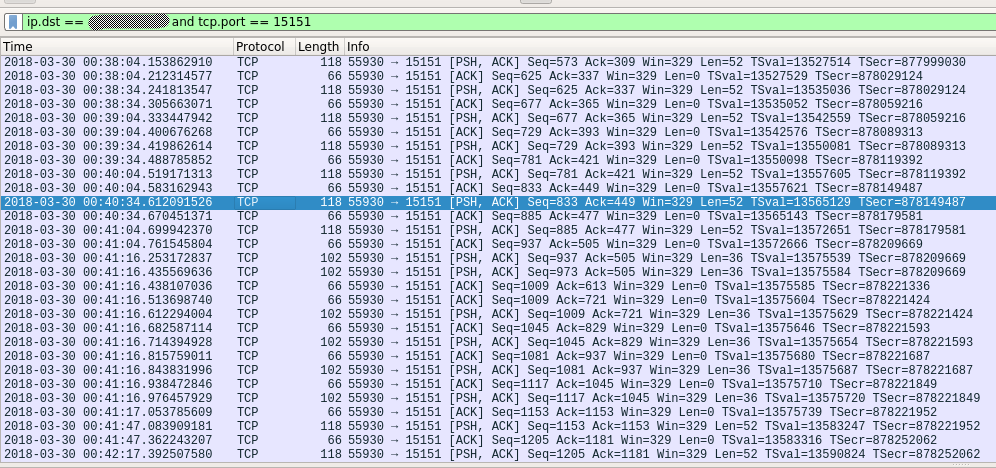
\includegraphics[scale=0.4]{sshheartbeatpackage.png}
	\caption{ssh心跳包}
	\label{fig:sshheartbeatpackage}
\end{figure}


\subsection{Permission denied (publickey)}

在ssh登陆机器时,提示Permission denied (publickey)。可以尝试的方法,在连接命令中加上-vvv参数,观察详细的调试输出:

\begin{lstlisting}[language=Bash]
ssh -p 2222 -vvv hldev@10.0.0.22
\end{lstlisting}

设置文件夹对应的权限:

\begin{lstlisting}[language=Bash]
sudo chmod 700 .ssh
sudo chmod 600 .ssh/authorized_keys
\end{lstlisting}

登陆服务器观察相应的日志输出:

\begin{lstlisting}[language=Bash]
tail -f /var/log/auth.log
\end{lstlisting}

是不是服务器关闭了密码登陆?只能使用公钥认证登陆。后面检查确实如此,服务器端为了安全考虑,关闭了基于密码登录的方式,但是需要登录的主机并没有将自己的公钥拷贝到服务器上。所以服务器直接提示了Permission denied (publickey),解决的办法就是在服务器端暂时开启密码登录,在/etc/ssh/sshd\_config中调整配置:

\begin{lstlisting}[language=Bash]
#允许使用基于密钥认证的方式登陆
PubkeyAuthentication yes 
\end{lstlisting}


\subsection{Session时间}

在使用ssh的过程中,经常会遇到一会儿没有操作就自动断开了,不是非常方便。

\paragraph{ClientAliveInterval}

修改/etc/ssh/sshd\_config配置文件 ClientAliveInterval 300(默认为0),参数的是意思是每5分钟,服务器向客户端发一个消息,用于保持连接,使用service sshd reload 让其修改后生效。如果发现还是有问题,可以试着把300设置小一点,例如60。

\paragraph{ClientAliveCountMax}

另外,至于ClientAliveCountMax, 使用默认值3即可.ClientAliveCountMax表示服务器发出请求后客户端没有响应的次数达到一定值, 就自动断开。

\paragraph{ControlPersist 4h}

在./ssh/config中添加一行:

\begin{lstlisting}[language=Bash]
ControlPersist 4h
\end{lstlisting}

When used in conjunction with ControlMaster, specifies that the master connection should remain open in the background (waiting for future client connections) after the initial client connection has been closed. If set to no, then the master connection will not be placed into the background, and will close as soon as the initial client connection is closed. If set to yes or 0, then the master connection will remain in the background indefinitely (until killed or closed via a mechanism such as the “ssh -O exit”). If set to a time in seconds, or a time in any of the formats documented in sshd\_config, then the backgrounded master connection will automatically terminate after it has remained idle (with no client connections) for the specified time\footnote{\url{http://man.openbsd.org/ssh_config.5}}.现在你每次通过SSH与服务器建立连接之后,这条连接将被保持4个小时,即使在你退出服务器之后,这条连接依然可以重用,因此,在你下一次(4小时之内)登录服务器时,你会发现连接以闪电般的速度建立完成,这个选项对于通过scp拷贝多个文件提速尤其明显,因为你不在需要为每个文件做单独的认证了。

\subsection{代理转发}

\paragraph{本地转发Local Forward}

将本地机(客户机)的某个端口转发到远端指定机器的指定端口. 工作原理是这样的, 本地机器上分配了一个 socket 侦听 port 端口, 一旦这个端口上有了连接, 该连接就经过安全通道转发出去, 同时远程主机和 host 的 hostport 端口建立连接. 可以在配置文件中指定端口的转发. 只有 root 才能转发特权端口。应用实例可以参看\ref{paragraph:sshproxy}。

\begin{lstlisting}[language=Bash]
# Mac OS X端口转发
/usr/bin/ssh -g -L 2222:10.10.30.1:22222 127.0.0.1
# 接口服务器设置代理转发
ssh -g -L 7805:192.168.250.100:7805 10.10.1.32
\end{lstlisting}

有时在本地转发会遇到一些问题,比如Connection Refused。首先要确定本地要运行有ssh服务端,使用如下命令启动sshd:

\begin{lstlisting}[language=Bash]
# Mac OS X启动sshd
sudo /usr/bin/sshd
# Ubuntu启动sshd
sudo /etc/init.d/ssh
\end{lstlisting}

启动SSHD 的时候系统提示:Could not load host key: /etc/ssh/ssh\_ed25519\_key。新版的opensshd 中添加了Ed25519 做签名验证,而之前系统里没这个算法的证书,所以办法也很简单新生成下证书即可。

\begin{lstlisting}[language=Bash]
sudo ssh-keygen -t rsa -f /etc/ssh/ssh_host_rsa_key
sudo ssh-keygen -t dsa -f /etc/ssh/ssh_host_dsa_key
sudo ssh-keygen -t ecdsa -f /etc/ssh/ssh_host_ecdsa_key
ssh-keygen -t ed25519 -f /etc/ssh/ssh_host_ED25519_key
\end{lstlisting}


\subsection{ssh查看日志}

如果需要查看ssh日志,可在/etc/ssh/sshd\_config配置日志输出:

\begin{lstlisting}[language=Bash]
SysLogFacility LOCAL7
\end{lstlisting}

Facility:设施,是rsyslog引入的概念,从功能或者程序上对日志进行分类,并由专门的工作负责记录相对应的信息,分类有:

\begin{quote}
	auth(授权),authpriv,cron(定时任务),daemon(守护进程),kern(内核),lpr,mail(邮件相关),mark,news,security(安全),syslog,user,uucp,local0,local7。	
\end{quote}

多线程,多协议(udp/tcp/ssl/tls/relp);mysql,pgsql,oracle等多种关系数据中,强大的过滤器,可实现过滤系统信息中的任意部分。自定义输出格式。适用于企业级别日志记录需求。ssh配置文件配置后,在/etc/rsyslog.conf文件中作如下配置:

\begin{lstlisting}[language=Bash]
LOCAL7.*	/var/log/sshd.log
\end{lstlisting}




\section{VisualVM}

使用nmap扫描1099端口,看jstatd是否生效。



\section{Tool Set}

\subsection{ECS(Elastic Compute Service)}

配置内网ECS端口映射规则,在云服务器ECS-->网络和安全-->安全组-->配置规则-->添加安全组规则.

\subsection{shadowsocks}

启动ss服务器:

\begin{lstlisting}[language=Bash]
#可以查看启动日志
ssserver -c /home/ec2-user/shadowsocks.json
#后台启动
ssserver -c /home/ec2-user/shadowsocks.json -d start
\end{lstlisting}

Shadowsocks客户端操作:

\begin{lstlisting}[language=Bash]
sudo apt-get install python-pip
sudo apt-get install python-setuptools m2crypto
#安装Shadowsocks(Ubuntu/Fedora)
pip install shadowsocks
#前台启动
#可以看到实时的日志输出
#关闭终端后代理断开
sslocal -c /etc/shadowsocks/shadowsocks.json
#后台启动
sslocal -c /etc/shadowsocks/shadowsocks.json -d start
\end{lstlisting}

\subsection{youtube-dl}

YouTube视频一般是不能下载的,但是是国内访问YouTube比较慢,经常卡顿,所以可以使用youtube-dl工具下载YouTube视频:

\begin{lstlisting}[language=Bash]
#下载默认的视频格式
youtube-dl https://www.youtube.com/watch?v=SnHxKQiXrFU
#查看所有视频格式
youtube-dl -F https://www.youtube.com/watch?v=SnHxKQiXrFU
#下载指定清晰度的视频
#137为指定视频格式的编码format code
youtube-dl -f 137 https://www.youtube.com/watch?v=SnHxKQiXrFU
\end{lstlisting}

查看YouTube所有格式视频输出效果如图所示:

\begin{figure}[htbp]
	\centering
	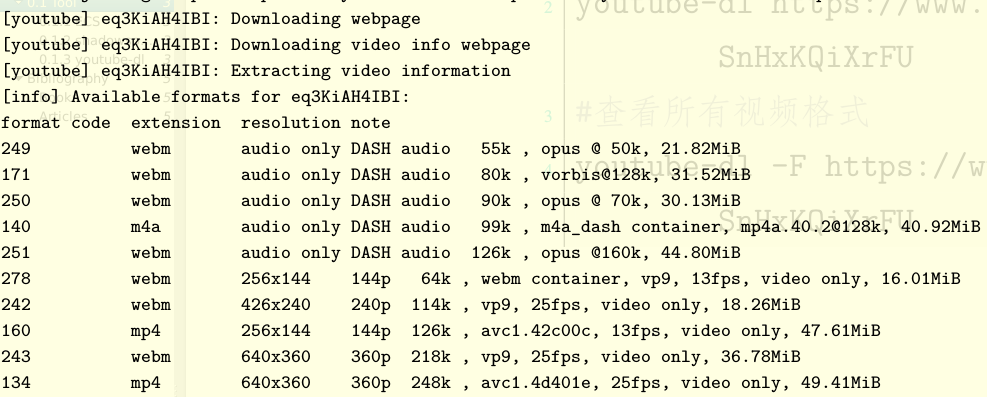
\includegraphics[scale=0.4]{checkyoubevideoformat.png}
	\caption{查看所有格式视频}
	\label{fig:checkyoubevideoformat}
\end{figure}




%----------------------------------------------------------------------------------------
%	CHAPTER 1
%----------------------------------------------------------------------------------------

\chapterimage{chapterhead2.pdf} % Chapter heading image


\subsection{Jenkins}

启动Jenkins提示Job for jenkins.service failed because the control process exited with error code. See "systemctl status jenkins.service" and "journalctl -xe" for details。多半是由于Java未安装或者安装后未指定Java路径。打开文件:

\begin{lstlisting}[language=bash]
#配置文件中指定Java路径
vim /etc/rc.d/init.d/jenkins
#启动Jenkins
service jenkins start
\end{lstlisting}

配置文件中指定Java路径如图所示。

\begin{figure}[htbp]
	\centering
	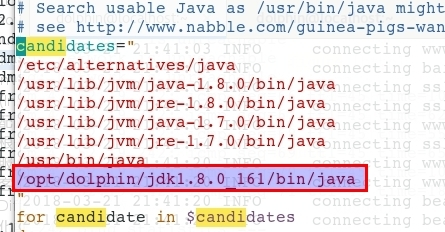
\includegraphics[scale=0.5]{specifyjavapath.jpg}
	\caption{指定Jenkins的Java路径}
	\label{fig:specifyjavapath}
\end{figure}

修改默认的端口号:

\begin{lstlisting}[language=bash]
vim /etc/sysconfig/jenkins
service jenkins restart
\end{lstlisting}

默认密码路径:

\begin{lstlisting}[language=bash]
#密码默认路径
vim /var/lib/jenkins/secrets/initialAdminPassword
vim {$home}/.jenkins/secrets/initialAdminPassword
\end{lstlisting}


\subsubsection{忘记登录密码}

忘记Jenkins登录密码,可以先禁用登录认证,进入Jenkins修改密码后,使用新密码登录,打开配置文件:

\begin{lstlisting}[language=bash]
vim /var/lib/jenkins/jenkins.config
\end{lstlisting}

删除与登录认证相关的配置:

\begin{lstlisting}[language=XML]
<useSecurity>true</useSecurity>  
<authorizationStrategy class="hudson.security.FullControlOnceLoggedInAuthorizationStrategy">  
	<denyAnonymousReadAccess>true</denyAnonymousReadAccess>  
</authorizationStrategy>  
<securityRealm class="hudson.security.HudsonPrivateSecurityRealm">  
	<disableSignup>true</disableSignup>  
	<enableCaptcha>false</enableCaptcha>  
</securityRealm>
\end{lstlisting}

1.重启Jenkins服务;

2.进入首页>“系统管理”>“Configure Global Security”;

3.勾选“启用安全”;

4.点选“Jenkins专有用户数据库”,并点击“保存”;

5.重新点击首页>“系统管理”,发现此时出现“管理用户”;

6.点击进入展示“用户列表”;

7.点击右侧进入修改密码页面,修改后即可重新登录。

\subsubsection{Jenkins中Gradle版本}

Jenkins中使用gradlew时,Gradle版本始终是某一个,但是build.gradle中和Jenkins中指定的却是另一个版本。

\begin{lstlisting}[language=bash]
#查看gradlew版本
./gradlew -v
#更新版本
gradle wrapper
\end{lstlisting}

\subsubsection{Jenkins中Gradle配置}

Jenkins中Gradle需要添加全局变量GRADLE\_USER\_HOME,在Jenkins->系统管理->系统设置->全局属性中,添加全局变量GRADLE\_USER\_HOME的路径要保证Jenkins用户有写入的权限,如图\ref{fig:gradleuserhome}所示.

\begin{figure}[htbp]
	\centering
	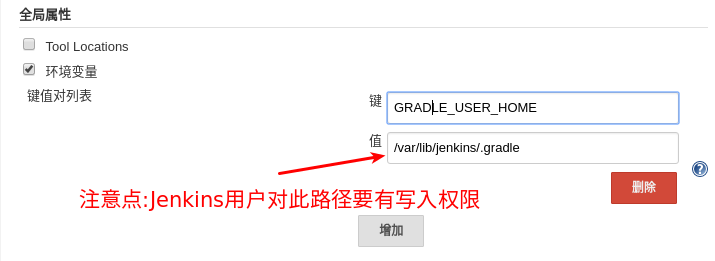
\includegraphics[scale=0.5]{gradleuserhome.png}
	\caption{指定Jenkins的Gradle用户路径}
	\label{fig:gradleuserhome}
\end{figure}


\subsubsection{Jenkins运行脚本}

Jenkins后台运行脚本时,需要使用setsid和设置BUILD\_ID=dontKillMe\footnote{\url{https://wiki.jenkins.io/display/JENKINS/ProcessTreeKiller}}.如下命令所示:

\begin{lstlisting}[language=bash]
count=`ps -ef | grep dolphin-web-${VERSION} | grep -v "grep" | wc -l`
if [ $count -lt 1 ]; then
	#使用setsid启动app
	#setsid在一个新的会话中运行命令
	#从而可以避开当前终端发出的HUP信号
	setsid ${JAVA_HOME}/bin/java -Xmx512M -Xms256M \
	-jar -Xdebug -Xrunjdwp:transport=dt_socket,suspend=n,server=y,address=5005	\
	${APP_PATH}/dolphin-web-${VERSION}.jar \
	--spring.config.location=${APP_PATH}/application.properties>/dev/null &
else
	echo "process aready exists!"
fi
\end{lstlisting}

也可以在Jenkins系统环境变量中设置BUILD\_ID变量,如图\ref{fig:jenkinsbuildidsetting}所示。

\begin{figure}[htbp]
	\centering
	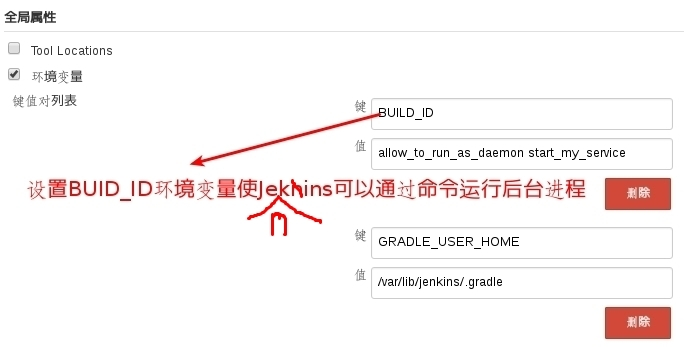
\includegraphics[scale=0.5]{jenkinsbuildidsetting.jpg}
	\caption{Jeknins全局变量}
	\label{fig:jenkinsbuildidsetting}
\end{figure}

Jenkins系统中添加执行脚本的时候,有一些命令是需要sudo权限和来执行的,可以在root权限下添加一下Jenkins账号的权限。如下命令所示:

\begin{lstlisting}[language=bash]
#打开sudoers文件
vim /etc/sudoers
\end{lstlisting}

在/etc/sudoers文件中添加如下内容:

\begin{lstlisting}[language=bash]
#可以不用输入密码
#直接以超级管理员权限执行ps命令和kill命令
jenkins ALL=NOPASSWD:/usr/bin/ps,/usr/bin/kill
\end{lstlisting}



\subsection{OpenVPN}

OpenVPN从2001年开始开发,使用的是C语言。此处使用的OpenVPN版本是2.4.1。如果使用Mac下的brew工具安装,则OpenVPN目录在:/usr/local/Cellar/openvpn/2.4.1,OpenVPN的配置文件在:/usr/local/etc/openvpn。目前OpenVPN能在Solaris、Linux、OpenBSD、FreeBSD、NetBSD、Mac OS X与Microsoft Windows以及Android和iOS上运行,并包含了许多安全性的功能。此处的服务器使用的是CentOS 7.3,客户端包含Fedora 24、Ubuntu 14.04、Ubuntu 16.04、Window 7、Windows 10。在OpenVPN网络中查看存活的主机:

\begin{lstlisting}[language=bash]
nmap -A -T4 10.0.0.*
\end{lstlisting}

\paragraph{安装(Install)}

安装基础包:

\begin{lstlisting}[language=bash]
sudo yum -y install openssl openssl-devel lzo openvpn easy-rsa --allowerasing
#手动安装
wget -c https://swupdate.openvpn.org/community/releases/openvpn-2.4.1.tar.gz
tar -zxvf openvpn-2.4.1.tar.gz
./configure
make && make install
\end{lstlisting}

LZO 是致力于解压速度的一种数据压缩算法,LZO 是 Lempel-Ziv-Oberhumer 的缩写。这个算法是无损算法,参考实现程序是线程安全的。 实现它的一个自由软件工具是lzop。最初的库是用 ANSI C 编写、并且遵从 GNU通用公共许可证发布的。现在 LZO 有用于 Perl、Python 以及 Java 的各种版本。代码版权的所有者是 Markus F. X. J. Oberhumer。如果没有安装easyrsa工具,使用如下命令安装:

\begin{lstlisting}[language=Bash]
#下载easy-rsa源码
wget -c https://github.com/OpenVPN/easy-rsa/archive/master.zip
#目录/etc/openvpn/easy-rsa/easyrsa3下拷贝默认配置
cp var.example vars
\end{lstlisting}


\paragraph{调整配置}

修改证书生成的配置文件:

\begin{lstlisting}[language=Bash]
set_var EASYRSA_REQ_COUNTRY     "CN"
set_var EASYRSA_REQ_PROVINCE    "Chongqing"
set_var EASYRSA_REQ_CITY        "Chongqing"
set_var EASYRSA_REQ_ORG "Three people"
set_var EASYRSA_REQ_EMAIL       "jiangtingqiang@gmail.com"
set_var EASYRSA_REQ_OU          "My Organizational"

set_var EASYRSA_KEY_SIZE        2048
\end{lstlisting}

\paragraph{生成根证书}

生成OpenVPN的根证书:

\begin{lstlisting}[language=Bash]
#清除之前生成的证书,重新生成;
./easyrsa clean-all
#生成root根证书
#证书路径:/etc/openvpn/easy-rsa/easyrsa3/pki/ca.crt
./easyrsa build-ca
\end{lstlisting}


\paragraph{生成服务器端证书}

生成服务器端证书命令如下:

\begin{lstlisting}[language=Bash]
# 指定服务端证书的文件名为server,可以任意改动
./easyrsa build-server-full server
\end{lstlisting}


\paragraph{生成客户端证书}

生成客户端证书端步骤如下:

\begin{lstlisting}[language=Bash]
./easyrsa build-client-full jiangxiaoqiang
\end{lstlisting}

PKI:Public Key Infrastructure公钥基础设施。生成请求:

\begin{lstlisting}[language=Bash]
./easyrsa gen-req dolphinfedora
\end{lstlisting}

输入PEM验证码。PEM - Privacy Enhanced Mail,打开看文本格式,以"-----BEGIN..."开头, "-----END..."结尾,内容是BASE64编码。
Apache和*NIX服务器偏向于使用这种编码格式.签约:

\begin{lstlisting}[language=Bash]
#切换到服务端生成rsa的目录
#导入req
./easyrsa import-req ~/client/easyrsa/easy-rsa-master/easyrsa3/pki/reqs/dolphinfedora.req dolphinfedora
#用户签约,根据提示输入服务端的ca密码
./easyrsa sign client dolphinfedora
\end{lstlisting}

PKI:Public Key Infrastructure公钥基础设施。输入PEM验证码。PEM - Privacy Enhanced Mail,打开看文本格式,以"-----BEGIN..."开头, "-----END..."结尾,内容是BASE64编码.查看PEM格式证书的信息:openssl x509 -in certificate.pem -text -noout。Apache和*NIX服务器偏向于使用这种编码格式.服务端生成的文件有:

\begin{tabular}{|c|p{5cm}|c|}
	\hline
	\multirow{1}{*}{文件名称}
	& \multicolumn{1}{c|}{说明(Purpose)} 
	& \multicolumn{1}{c|}{位置} \\			
	\cline{1-3}
	ca.crt  & 根证书(Root CA certificate)件 & Server+All Clients	\\
	\hline
	reqs/server.req  & &\\
	\hline
	reqs/dolphin.req  & &\\
	\hline
	private/ca.key & 根证书私钥(Root CA key) & key signing machine only\\
	\hline
	private/server.key && \\
	\hline
	issued/server.crt & 服务器证书Server Certificate & server only\\
	\hline
	issued/dolphin.crt && \\
	\hline
	dh.pem & Diffie Hellman parameters & server only \\
	\hline
\end{tabular}

客户端生成的文件有:

\begin{tabular}{|c|p{8cm}|c|}
	\hline
	\multirow{1}{*}{序号}
	& \multicolumn{1}{c|}{名称}  \\			
	\cline{1-2}
	private/dolphinclient.key  & \\
	\hline
	reqs/sdolphinclient.req & \\
	\hline
\end{tabular}

拷贝出客户端证书文件:

\begin{lstlisting}[language=Bash]
cp easyrsa/easy-rsa-master/easyrsa3/pki/ca.crt ~/dolphinfedora/
cp easyrsa/easy-rsa-master/easyrsa3/pki/issued/dolphinfedora.crt ~/dolphinfedora/
cp ~/client/easyrsa/easy-rsa-master/easyrsa3/pki/private/dolphinfedora.key ~/dolphinfedora/
\end{lstlisting}


启动OpenVPN:

\begin{lstlisting}[language=Bash]
sudo openvpn server.conf
# Mac下启动OpenVPN
sudo /usr/local/Cellar/openvpn/2.4.1/sbin/openvpn /usr/local/etc/openvpn/client.conf
# 需要以后台交互方式启动时
screen sudo openvpn client.conf
\end{lstlisting}

客户端端配置如下:

\begin{lstlisting}[language=Bash]
client         #指定当前VPN是客户端
dev tun        #必须与服务器端的保持一致
proto udp      #必须与服务器端的保持一致
#指定连接的远程服务器的实际IP地址和端口号
remote 192.168.1.106 1194      
#断线自动重新连接
#在网络不稳定的情况下(例如:笔记本电脑无线网络)非常有用
resolv-retry infinite
nobind         #不绑定特定的本地端口号
persist-key
persist-tun
ca ca.crt      #指定CA证书的文件路径
cert client1.crt       #指定当前客户端的证书文件路径
key client1.key    #指定当前客户端的私钥文件路径
ns-cert-type server      #指定采用服务器校验方式
#如果服务器设置了防御DoS等攻击的ta.key
#则必须每个客户端开启;如果未设置,则注释掉这一行;
tls-auth ta.key 1     
comp-lzo              #与服务器保持一致
#指定日志文件的记录详细级别,可选0-9,等级越高日志内容越详细
verb 3                
\end{lstlisting}

配置ns-cert-type(Netscape Cert Type)指定为server主要是防止中间人攻击(Man-in-the-Middle Attack)。在服务端做如下配置:

\begin{lstlisting}[language=Bash]
nsCertType server
\end{lstlisting}

\paragraph{生成Diffle Hellman参数}

生成Diffle Hellman参数命令如下:

\begin{lstlisting}[language=Bash]
./easyrsa gen-dh
\end{lstlisting}

\paragraph{初始化配置文件}

初始化配置文件如下:

\begin{lstlisting}[language=Bash]
#拷贝示例配置到配置目录
cp /usr/share/doc/openvpn-2.4.4/sample/sample-config-files/server.conf /etc/openvpn
\end{lstlisting}

拷贝server.crt/ca.cert等文件到配置目录.


\paragraph{生成ta.key}

使用如下命令生成ta.key:

\begin{lstlisting}[language=Bash]
openvpn --genkey --secret ta.key
\end{lstlisting}

启动服务端:

\begin{lstlisting}[language=Bash]
openvpn --config /etc/openvpn/server.conf
\end{lstlisting}

\paragraph{拷贝客户端文件}

将服务器生成的客户端文件拷贝到客户端:

\begin{lstlisting}[language=Bash]

\end{lstlisting}


\subsection{fastDFS}

启动tracker server:

\begin{lstlisting}[language=Bash]
/usr/bin/fdfs_trackerd /etc/fdfs/tracker.conf
\end{lstlisting}

启动storaged server:

\begin{lstlisting}[language=Bash]
/usr/bin/fdfs_storaged /etc/fdfs/storage.conf
\end{lstlisting}

\section{Nginx}

安装配置好nginx服务器后默认目录是/usr/share/nginx/html。nginx模块一般被分成三大类:handler、filter和upstream。Mac下Nginx配置文件的路径为:/usr/local/etc/nginx/nginx.conf。

\subsection{X-Forwarded-For}

X-Forwarded-For是一个HTTP扩展头部。HTTP/1.1(RFC 2616)协议并没有对它的定义,它最开始是由 Squid 这个缓存代理软件引入,用来表示 HTTP 请求端真实 IP。如今它已经成为事实上的标准,被各大 HTTP 代理、负载均衡等转发服务广泛使用,并被写入 RFC 7239(Forwarded HTTP Extension)标准之中。在默认情况下,Nginx并不会对X-Forwarded-For头做任何的处理,除非用户使用proxy\_set\_header参数设置:

\begin{lstlisting}[language=bash]
proxy_set_header X-Forwarded-For $proxy_add_x_forwarded_for;
\end{lstlisting}

X-Forwarded-For请求头格式:

\begin{lstlisting}[language=bash]
X-Forwarded-For: IP0, IP1, IP2
\end{lstlisting}

XFF 的内容由「英文逗号 + 空格」隔开的多个部分组成,最开始的是离服务端最远的设备 IP,然后是每一级代理设备的 IP。

\subsection{Nginx获取真实IP}

Nginx作为HTTP代理转发前端时,后端服务无法获知前端访问客户的IP地址。要获取客户端IP,需要将http\_realip\_module编译进入Nginx中。查看Nginx安装了哪些模块,使用如下命令:

\begin{lstlisting}[language=bash]
nginx -V
\end{lstlisting}

在命令的输出结果中,可以看到Nginx的版本,Nginx的编译参数,和Nginx已经包含有哪些模块。此处显示已经编译了http\_realip\_module模块。在服务器上的项目中使用的tengine,经过查看是没有编译http\_realip\_module模块,从tengine官网上下载好源码,输入如下命令进行编译:

\begin{lstlisting}[language=bash]
# 在Ubuntu 14.04 LTS下安装pcre依赖
# pcre:Perl Compatible Regular Expressions
sudo apt-get install libpcre3 libpcre3-dev
# 指定预编译参数,仅仅指定路径
sudo ./configure --prefix=/opt/tengine
# 将realip模块编译进入
sudo ./configure --prefix=/opt/tengine --with-http_realip_module
# 编译
sudo make
# 安装
sudo make install
./configure --prefix=/usr/local/tengine-2.1.2 --with-openssl=/Users/dolphin/source/openssl
\end{lstlisting}

不指定prefix,则可执行文件默认放在/usr/local/bin,库文件默认放在/usr/local/lib,配置文件默认放在/usr/local/etc。其它的资源文件放在/usr /local/share。
你要卸载这个程序,要么在原来的make目录下用一次make uninstall(前提是make文件指定过uninstall),要么去上述目录里面把相关的文件一个个手工删掉。
指定prefix,直接删掉一个文件夹就够了,这也是制定prefix一个比较方便的地方。在编译时,还需要指定pcre的版本,因为Ubuntu 16.04 LTS里有时安装有pcre 3,而部署的电脑上不一定安装有pcre 3,而且pcre 3的源码不容易找到。所以编译命令如下:

\begin{lstlisting}[language=bash]
# 将realip模块编译进入,并指定pcre
sudo ./configure --prefix=/opt/tengine --with-http_realip_module --with-pcre=/root/software/pcre-8.40 --with-openssl=/root/software/openssl-OpenSSL_1_1_0e --without-http_gzip_module

./configure --prefix=/opt/tengine --with-http_realip_module --with-pcre=/root/software/pcre-8.40  --without-http_gzip_module

#本机编译(不成功)
./configure --prefix=/opt/tengine --with-http_realip_module --with-pcre=/home/hldev/Downloads/pcre-8.40 --with-openssl=/home/hldev/Downloads/openssl-OpenSSL_1_0_1e --without-http_gzip_module

#本机编译(成功)
-prefix=/opt/tengine --with-http_realip_module --with-pcre=/home/hldev/Downloads/pcre-8.40 --with-openssl=/home/hldev/software/openssl-OpenSSL_1_0_2g --without-http_gzip_module

# 构建程序
make

#安装程序
make install

#服务器
./configure --prefix=/opt/tengine

./configure: error: SSL modules require the OpenSSL library.
You can either do not enable the modules, or install the OpenSSL library
into the system, or build the OpenSSL library statically from the source
with nginx by using --with-openssl=<path> option.


\end{lstlisting}

其中--with-pcre表示pcre(Perl Compatible Regular Expressions)的源代码目录。在编译时,还需要注意openssl的版本,本地电脑版本是1.0.2g,服务端的版本是1.0.1e。服务器端编译Nginx的一个命令:

\begin{lstlisting}[language=bash]
./configure --prefix=/opt/tengine --with-openssl=/usr/local/src/openssl-OpenSSL_1_0_2g/ --without-http_gzip_module --with-pcre=/usr/local/src/pcre-8.40/
\end{lstlisting}

这里编译的时候有一个小细节需要注意,需要将源码包存放到/usr/local/src目录下。一直没有编译成功也许是这个小小的细节,开始时是将源码包随意存放的一个目录。以上编译的命令没有包含Zlib,也没有包含http\_realip\_module模块。最终的编译命令如下:

\begin{lstlisting}[language=bash]
./configure --prefix=/opt/tengine --with-openssl=/usr/local/src/openssl-OpenSSL_1_0_2g/ --with-pcre=/usr/local/src/pcre-8.40/ --with-zlib=/usr/local/src/zlib-1.2.11 --with-http_realip_module 
\end{lstlisting}

编译完毕之后,输入如下命令:

\begin{lstlisting}[language=bash]
# 查看Tengine版本、模块信息,编译时所使用的参数
./nginx -V
\end{lstlisting}

即可看到http\_realip\_module已经编译到Nginx中了。Nginx的http realip module等于Apache的mod\_rpaf,用于接受前端发来的IP head信息,从获取到真实的用户IP。将获取真实IP的模块编译进入Nginx后,还需要在对应的http、server、location中加入以下参数:

\begin{lstlisting}[language=bash]
#指令是告诉nginx,10.10.1.11是我们的反向代服务器
#不是真实的用户IP
set_real_ip_from 10.10.1.11;
#告诉nginx真正的用户IP是存在
#X-Forwarded-For请求头中
real_ip_header X-Real-IP;
\end{lstlisting}

其中set\_real\_ip\_from可以指定某个网段。这个指令指定信任的代理IP,它们将会以精确的替换IP转发。0.8.22后可以指定Unix sockets。real\_ip\_header设置需要使用哪个头来确定替换的IP地址。由于项目中使用的Nginx作为反向代理,所以配置如下:

\begin{lstlisting}[language=bash]
location /inapi {
proxy_pass http://localhost:28080;
proxy_set_header X-Real-IP $remote_addr;
proxy_redirect off;
}
\end{lstlisting}

在另一台电脑上访问服务端,在后端根据新添加的Header获取到的IP地址如图\ref{fig:nginxgetrealip}所示:

\begin{figure}[htbp]
	\centering
	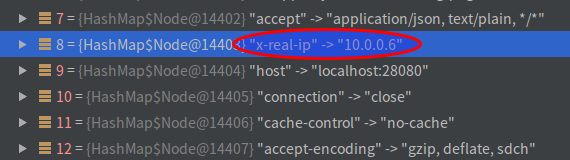
\includegraphics[scale=0.6]{nginxgetrealip.png}
	\caption{Nginx获取用户真实访问IP}
	\label{fig:nginxgetrealip}
\end{figure}

此处获取到的IP是用户的真实IP,而不是反向代理服务器的IP。

\subsection{Nginx并发(Nginx Concurrent)}

如何设置能限制某个IP某一时间段的访问次数是一个让人头疼的问题,特别面对恶意的ddos攻击的时候。其中CC攻击(Challenge Collapsar)是DDOS(分布式拒绝服务)的一种,也是一种常见的网站攻击方法,攻击者通过代理服务器或者肉鸡向向受害主机不停地发大量数据包,造成对方服务器资源耗尽,一直到宕机崩溃。

cc攻击一般就是使用有限的ip数对服务器频繁发送数据来达到攻击的目的,Nginx可以通过HttpLimitReqModule和HttpLimitZoneModule配置来限制ip在同一时间段的访问次数来防cc攻击。

HttpLimitReqModule用来限制连单位时间内连接数的模块,使用limit\_req\_zone和limit\_req指令配合使用来达到限制。一旦并发连接超过指定数量,就会返回503错误。limit\_req\_zone 用来限制单位时间内的请求数,即速率限制,采用的漏桶算法 “leaky bucket”。

\begin{lstlisting}[language=bash]
http {
limit_conn_log_level error;
limit_conn_status 503;
#Zone=one或allips表示设置了
#名为“one”或“allips”的存储区
#大小为10兆字节
limit_conn_zone $binary_remote_addr zone=one:10m;
limit_conn_zone $server_name zone=perserver:10m;
#rate=10r/s 的意思是允许1秒钟不超过1000个请求
limit_req_zone $binary_remote_addr zone=allips:100m rate=1000r/s;  
server {
limit_conn one 100;
limit_conn perserver 3000;
limit_req zone=allips  burst=5  nodelay;
}
}
\end{lstlisting}

HttpLimitConnModule用来限制单个ip的并发连接数,使用limit\_zone和limit\_conn指令,这两个模块的区别前一个是对一段时间内的连接数限制,后者是对同一时刻的连接数限制。

\subsection{URI长度限制}

在Http1.1协议中并没有提出针对URL的长度进行限制,RFC协议里面是这样描述的,HTTP协议并不对URI的长度做任何的限制,服务器端必须能够处理任何它们所提供服务多能接受的URI,并且能够处理无限长度的URI,如果服务器不能处理过长的URI,那么应该返回414状态码。接触的最多的服务器类型就是Nginx和Tomcat,对于url的长度限制,它们都是通过控制http请求头的长度来进行限制的,nginx的配置参数为large\_client\_header\_buffers,tomcat的请求配置参数为maxHttpHeaderSize。

\begin{lstlisting}[language=bash]
# Nginx配置HTTP请求头长度
client_header_buffer_size 2048k;
\end{lstlisting}

项目采用Spring Boot,所使用的Tomcat为内嵌的Tomcat。在application.properties中,增加如下配置:

\begin{lstlisting}[language=bash]
#单位为KB,如果没有指定,默认为8192(8KB)
server.max-http-header-size=1024
\end{lstlisting}

奇怪的是,在本机设置的1024KB可以查询,部署到服务器上,参数必须再调大才能够查询,否则提示请求头太大的错误。真的遇到鬼了。在不同的操作系统上单位不一样吗?见鬼

\subsection{开启Gzip压缩}

Nginx开启Gzip压缩配置如下:

\begin{lstlisting}[language=Bash]
gzip on;
gzip_min_length 1k;
gzip_buffers 4 16k;
gzip_comp_level 2;
gzip_types application/javascript application/json text/plain application/x-javascript text/css application/xml text/javascript application/x-httpd-php image/jpeg image/gif image/png;
gzip_vary off;
gzip_disable "MSIE [1-6]";
\end{lstlisting}

用curl测试是否开启了压缩:

\begin{lstlisting}[language=Bash]
curl -I -H "Accept-Encoding: gzip, deflate" "http://creditsystem.test/main"
curl -I -H "Accept-Encoding: gzip, deflate" "http://10.10.1.11/main"
\end{lstlisting}

-I选项与-header选项是等价的,表示只打印出HTTP头部。开启压缩成功后,可以看到一句:Content-Encoding: gzip。

\subsection{Nginx与爬虫(Nginx Anti-Spider)}

Nginx限制统一IP每分钟访问的次数:

\begin{lstlisting}[language=Bash]
limit_req_zone $binary_remote_addr zone=one:3m rate=1r/s;
limit_req_zone $binary_remote_addr $uri zone=two:3m rate=1r/s;
limit_req_zone $binary_remote_addr $request_uri zone=thre:3m rate=1r/s;      
\end{lstlisting}


可以根据客户端的 user-agents 首部字段来阻止指定的爬虫爬取我们的网站.

\subsection{Nginx配置}

简单的配置:

\begin{lstlisting}[language=bash]
user www-data;
worker_processes 4;
pid /run/nginx.pid;

events {
	worker_connections 768;
}

http {
	server{
		listen 80;
		# 定义网站默认根目录
		root /opt/dolphin/frontend/dist;
		
		location /api {
			proxy_pass http://localhost:8011;
		}
		
		location / {
			root /opt/dolphin/frontend/dist;
			index index.html;
		} 
	}
}
\end{lstlisting}

Nginx部署React项目的简单配置如图\ref{fig:nginxreactconfig}所示。

\begin{figure}[htbp]
	\centering
	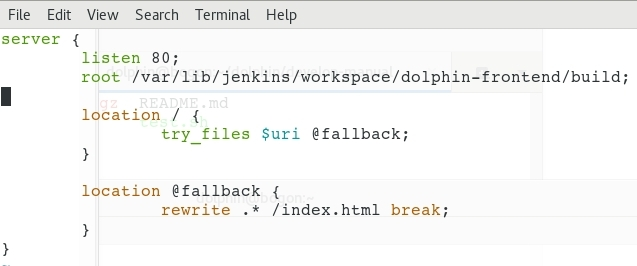
\includegraphics[scale=0.6]{nginxreactconfig.jpg}
	\caption{Nginx React简单配置}
	\label{fig:nginxreactconfig}
\end{figure}

在0.7以后的版本中加入了一个try\_files指令,配合命名location,可以部分替代原本常用的rewrite配置方式。其作用是按顺序检查文件是否存在,返回第一个找到的文件或文件夹(结尾加斜线表示为文件夹),如果所有的文件或文件夹都找不到,会进行一个内部重定向到最后一个参数。此处配置如果\$url不存在,则内部重定向到 @fallback。

\subsection{负载均衡(Load Balance)}

Nginx的负载均衡配置,在主机(10.10.1.12)出现问题时,Nginx会自动切换到备机(10.10.1.13),当主机恢复服务后,Nginx会自动切换回主机:

\begin{lstlisting}[language=bash]
upstream backend{
	server 10.10.1.12:28080;
	server 10.10.1.13:28080 backup;
}
\end{lstlisting}

而反向代理实际意义就是把请求转发, 使用的时候用 proxy\_pass 实现.
反向代理与正向代理都是用 proxy\_pass 来实现的, 使用起来没有太大的区别, 本质上都是转发网络请求.
反向代理一般指服务器将请求转发到内部网络, 这样可以防范外网直接请求内网带来的网络风险。

\subsection{阻止请求}

项目中有一个张表有700W+数据,是采用like匹配,like匹配无法利用索引,只能全表扫描,有时会有爬虫不断的请求此接口,导致数据库压力不断增大。为了临时应对,临时限制此接口的请求。如下代码片段所示:

\begin{lstlisting}[language=bash]
location /dolphin/api {
	#匹配类似于/dolphin/api/test/reg?id=1的url
	#不阻止形如/dolphin/api/test/reg请求
	if ( $args ~ id= ) {
		return 403;
	}
	proxy_pass http://localhost:8011;
	proxy_redirect off;
}
\end{lstlisting}


\subsection{超时转发}

当一个请求到达后端机器,后端机器因某些原因(load高等等)响应变慢导致超时的时候,Nginx会把这个请求转发到另外的后端机器上.The proxy\_next\_upstream directive is a configuration directive to control re-request from a group of upstream servers by a proxy\_pass if request to one of them fails. 

\begin{lstlisting}
server {
location / {
proxy_pass http://backends;
proxy_next_upstream error timeout http_404;
}
}
\end{lstlisting}

proxy\_next\_upstream在nginx中是默认打开的。参数值timeout,这个参数代表如果超时,则尝试其他节点。


\subsection{常见问题}

\paragraph{open() "/opt/tengine/conf/nginx.conf" failed (2: No such file or directory)}

以上的路径是编译时Nginx配置文件的路径,如果在启动时不指定配置文件和日志文件的路径,那么Nginx默认使用的时编译时的文件路径,但是在这里已经将编译文件移动到另外的文件夹里面了,所以需要显示的指定配置文件的路径:

\begin{lstlisting}[language=bash]
#启动Nginx(测试环境)
/opt/app/local/tengine/sbin/nginx -c /opt/app/local/tengine/conf/nginx.conf -p /opt/app/local/tengine
#启动Nginx(正式环境)
/home/app/local/tengine/sbin/nginx -c /home/app/local/tengine/conf/nginx.conf -p /home/app/local/tengine
\end{lstlisting}

也可以指定prefix文件目录,这样就会更改默认的Nginx主目录了:

\begin{lstlisting}[language=bash]
#重新加载配置(测试环境)
/opt/app/local/tengine/sbin/nginx -s reload -p /opt/app/local/tengine
/opt/app/local/tengine/sbin/nginx -c /opt/app/local/tengine/conf/nginx.conf -p /opt/app/local/tengine
/opt/home/local/tengine/sbin/nginx -c /home/app/local/tengine/conf/nginx.conf -p /home/app/local/tengine
\end{lstlisting}

其中opt目录是编译时指定的目录,/opt/app/local是新的目录,用p参数指定新目录即可。同理,在刷新配置的时候也需要显示的指定Nginx的主目录:

\begin{lstlisting}[language=bash]
#重新加载配置(正式环境Nginx Reload)
/home/app/local/tengine/sbin/nginx -p /home/app/local/tengine -s reload
./nginx -p /home/app/local/tengine -V
\end{lstlisting}

4C:CC:6A:7C:C3:CF
D8:CB:8A:8A:CD:15

\paragraph{error while loading shared libraries: libpcre.so.3: cannot open shared object file}

找不到libpcre.so.3文件,在本机搜索了之后,发现文件在目录下:

\begin{lstlisting}[language=bash]
/lib/i386-linux-gnu/libpcre.so.3
/lib/x86_64-linux-gnu/libpcre.so.3
\end{lstlisting}

\paragraph{error while loading shared libraries: libssl.so.1.0.0: cannot open shared object file}

有可能是由于openssl库的位置不对导致的,可以尝试创建软链接解决:

\begin{lstlisting}[language=bash]
ln -s /usr/local/lib64/libssl.so.1.1 /usr/lib64/libssl.so.1.1  
ln -s /usr/local/lib64/libcrypto.so.1.1 /usr/lib64/libcrypto.so.1.1  
\end{lstlisting}

.so 为共享库,是shared object,用于动态连接的,和dll差不多。openssl:多用途的命令行工具,各功能分别使用子命令实现,libcrypto:公共加密库(存放了各种加密算法),libssl:ssl协议的实现。在Ubuntu下可以通过如下命令安装libssl.so.1.0.0:

\begin{lstlisting}[language=bash]
sudo apt-get install libssl1.0.0:amd64
sudo apt-get install libssl1.0.0 libssl-dev

#查看OpenSSL版本
openssl version

#查看系统中对libssl
find / -name libssl.s0*

# 列出openssl包
yum list \*openssl\*
\end{lstlisting}

不过此处不能通过命令安装,只能通过源码编译安装。这里有包: \url{https://pkgs.org/download/libssl1.0.0}。查看当前操作系统支持的openssl:

\begin{lstlisting}[language=bash]
yum --showduplicates list openssl
\end{lstlisting}

寻找包含libssl.so.1.0.0的安装包:

\begin{lstlisting}[language=bash]
yum provides */libssl.so.1.0.0
\end{lstlisting}

在http://rpm.pbone.net/上搜索 openssl1-1.0.0 ,搜到openssl1-1.0.0-4.fc24.x86\_64.rpm。

\chapter{Gradle}

一般在Mac下Gradle的安装路径为:/usr/local/Cellar/gradle/3.2.1/libexec,在Mac的Intellij Idea指定Gradle路径时,即用此路径。

\begin{lstlisting}
${PROGRAM_DEVELOP_PATH_BACKEND}/gradlew -p ${PROGRAM_DEVELOP_PATH_BACKEND}/cc-web-boot -x test build --info
\end{lstlisting}

info参数会输出详细的log信息,便于问题定位.

\section{基础}

Gradle使用的Groovy语言,Groovy语言字符串的表示形式很多,有一些细微的区别:

\begin{lstlisting}
def a = '单引号形式'
def b = "双引号形式,${v}"
def c = '''三个单引号形式
支持多行
不支持占位符'''
def d = """三个双引号形式
支持多行
支持占位符,${v}"""
def e = /反斜杠形式
支持多行
支持占位符,${v}/
def f = $/美刀反斜杠形式
支持多行
支持占位符,${v}/$
\end{lstlisting}

建议使用'和"这两种形式。单引号''中的内容严格对应Java中的String,不对\$符号进行转义。双引号""的内容则和脚本语言的处理有点像,如果字符中有\$号的话,则它会\$表达式先求值。三个引号'''xxx'''中的字符串支持随意换行。

\subsection{引用本地文件}

有时候项目依赖的可能不是公布在网络上的一个公共库,可能只是一个闭源的jar包,只是一个本地文件而已。Gradle中引用本地文件写法如下:

\begin{lstlisting}[language=Java]
def ccDataLibs = fileTree(dir: "$rootDir/cc-data/lib", include: '*.jar')

dependencies {
compile ccDataLibs
}
\end{lstlisting}

dir表示文件所在目录,include表示包含哪些文件。

\subsection{Gradle Properties支持}

Gradle支持三种Properties, 这三种Properties的作用域和初始化阶段都不一样:

\textbf{System Properties:}
可通过gradle.properties文件,环境变量或命令行-D参数设置,可在setting.gradle或build.gradle中动态修改,在setting.gradle中的修改对buildscript block可见;所有工程可见,不建议在build.gradle中修改。多子工程项目中,子工程的gradle.properties会被忽略掉,只有root工程的gradle.properties有效。

\textbf{Project Properties:}可通过gradle.properties文件,环境变量或命令行-P参数设置,优先级是:
可在build.gradle中动态修改,但引用不存在的project properties会立即抛错,
动态修改过的project properties在buildscript block中不可见。

\textbf{Project ext properties:}可在项目的build.gradle中声明和使用,本工程和子工程可见,不能在setting.gradle中访问,如果有多处设置,加载次序如下(注意:gradle 2.0是这样的, 1.10~1.12有bug), 后面的覆盖前面的设置。

\begin{itemize}
	\item {from gradle.properties located in project build dir.}
	\item {from gradle.properties located in gradle user home.}
	\item {from system properties, e.g. when -Dsome.property is used in the command line.}
	\item {setting.gradle}
	\item {build.gradle}
\end{itemize}


\subsection{执行流程}

There is a one-to-one relationship between a Project and a "build.gradle" file. During build initialisation, Gradle assembles a Project object for each project which is to participate in the build, as follows:

Create a Settings instance for the build.
Evaluate the "settings.gradle" script, if present, against the Settings object to configure it.
Use the configured Settings object to create the hierarchy of Project instances.
Finally, evaluate each Project by executing its "build.gradle" file, if present, against the project. The projects are evaluated in breadth-wise order, such that a project is evaluated before its child projects. This order can be overridden by calling evaluationDependsOnChildren() or by adding an explicit evaluation dependency using evaluationDependsOn(String).

\subsection{默认JVM}

在Intellij Idea中首次导入Gradle项目时,可能提示未设置Gradle JVM,此时在项目初始选择页面选择Configure > Project Defaults > Project Structure,在项目Structure中设置JVM即可。

\subsection{Repositories}

Gradle默认每次编译或者刷新(Refresh)都会Resolve Dependencies,每次都会去进行网络请求。可以通过Wireshark抓包来验证是否有网络请求以及请求的具体地址,从图中可以看出Gradle Resolve时的请求地址,如果没有调整请求地址,Gradle会使用默认的Maven仓库的地址或JCenter地址,众所周知,国访问Maven仓库非常慢,导致Gralde一直卡在Resolve Dependencies阶段,具体如图\ref{fig:wiresharkcapturegradlerequest}所示。

\begin{figure}[htbp]
	\centering
	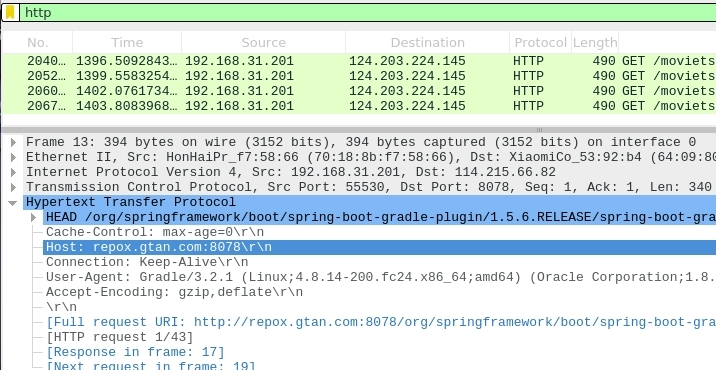
\includegraphics[scale=0.5]{wiresharkcapturegradlerequest.jpg}
	\caption{Wireshark查看Gradle Resolve请求}
	\label{fig:wiresharkcapturegradlerequest}
\end{figure}


如果访问JCenter很慢,光是这个步骤说不定就要十几分钟。解决方法是在Project Preferences的Gradle那里启用Offline work。注意这样之后当你添加了新的dependencies,它是不会去自动下载的,也就是说报错。需要进入项目目录运行gradlew手动同步,或是临时在Preferences那里禁用Offline work。也可以设置国内的源,在home目录.gradle文件夹中新建init.gradle文件,并在文件中输入如下内容,指定默认的国内源的地址,加速依赖包下载速度:

\begin{lstlisting}
allprojects{
repositories {
def ALIYUN_REPOSITORY_URL = 'http://maven.aliyun.com/nexus/content/groups/public'
def ALIYUN_JCENTER_URL = 'http://maven.aliyun.com/nexus/content/repositories/jcenter'
all { ArtifactRepository repo ->
if(repo instanceof MavenArtifactRepository){
def url = repo.url.toString()
if (url.startsWith('https://repo1.maven.org/maven2')) {
project.logger.lifecycle "Repository ${repo.url} replaced by $ALIYUN_REPOSITORY_URL."
remove repo
}
if (url.startsWith('https://jcenter.bintray.com/')) {
project.logger.lifecycle "Repository ${repo.url} replaced by $ALIYUN_JCENTER_URL."
remove repo
}
}
}
maven {
url ALIYUN_REPOSITORY_URL
url ALIYUN_JCENTER_URL
}
}
}
\end{lstlisting}

在Gradle构建标本build.gradle里,经常会看到如下脚本:

\begin{lstlisting}[language=Java]
repositories {
maven {
url 'http://www.eveoh.nl/files/maven2'
}
maven {
url 'http://repox.gtan.com:8078'
}
mavenCentral()
jcenter()
maven { 
url 'http://repo.spring.io/plugins-release' 
}
}
\end{lstlisting}

总的来说,只有两个标准的Android library文件服务器:JCenter 和 Maven Central。起初,Android Studio 选择Maven Central作为默认仓库。如果你使用老版本的Android Studio创建一个新项目,mavenCentral()会自动的定义在build.gradle中。但是Maven Central的最大问题是对开发者不够友好。上传library异常困难。上传上去的开发者都是某种程度的极客。同时还因为诸如安全方面的其他原因,Android Studio团队决定把默认的仓库替换成JCenter。正如你看到的,一旦使用最新版本的Android Studio创建一个项目,JCenter()自动被定义,而不是mavenCentral()。mavenCentral()表示依赖是从Central Maven 2 仓库中获取的,库的地址是\url{https://repo1.maven.org/maven2}。JCenter表示依赖是从Bintary’s JCenter Maven 仓库中获取的,仓库的地址是\url{https://jcenter.bintray.com},Bintray是一家提供全球企业软件开发包托管的商业公司。

\subsection{常见问题}

\paragraph{could not find method compile()}

gradle项目配置中引用java插件。


\paragraph{Could not find or load main class org.gradle.wrapper.GradleWrapperMain}

运行gradlew脚本时,出现错误:Could not find or load main class org.gradle.wrapper.GradleWrapperMain,安装gradle后运改gradle wrapper命令修复。  


\paragraph{Gradle找不到Tasks}

有时在使用Gradle命令编译时找不到相应到任务(Tasks)。比如在部署脚本在project/script/deploy目录下,当在此目录下运行脚本时,会提示在项目目录deploy下找不到任务。命令如下:

\begin{lstlisting}[language=Bash]
${PROGRAM_DEVELOP_PATH_BACKEND}/gradlew copyTask -x test
\end{lstlisting}

此时就需要指定项目的路径,将命令调整为:

\begin{lstlisting}[language=Bash]
${PROGRAM_DEVELOP_PATH_BACKEND}/gradlew -p ${PROGRAM_DEVELOP_PATH_BACKEND} copyTask -x test
\end{lstlisting}

p参数指定项目的路径。在不同目录下面执行gradle tasks命令,可以看到不同的任务,当在/project/script/deploy目录下执行gradle tasks命令时,是看不到copyTask命令的,但是在项目的根目录下执行是可以看到copyTasks任务,如图\ref{fig:copyTasks}所示。

\begin{figure}[htbp]
	\centering
	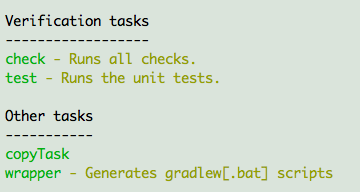
\includegraphics[scale=0.7]{copytasks.png}
	\caption{Gradle查看Tasks}
	\label{fig:copyTasks}
\end{figure}

\section{Gradle对象}

\subsection{属性(Properties)}

\subsubsection{Extra Properties}

extra属性一般用于定义常量,All extra properties\footnote{\url{https://docs.gradle.org/current/javadoc/org/gradle/api/Project.html\#extraproperties}} must be defined through the "ext" namespace. Once an extra property has been defined, it is available directly on the owning object (in the below case the Project, Task, and sub-projects respectively) and can be read and updated. Only the initial declaration that needs to be done via the namespace.

\begin{lstlisting}[language=Java]
buildscript {
ext {
springBootVersion = '1.4.5.RELEASE'
jacksonVersion = '2.8.7'
springfoxVersion = '2.6.1'
poiVersion = "3.14"
aspectjVersion = '1.7.4'
}
}
\end{lstlisting}

Reading extra properties is done through the "ext" or through the owning object.


ext.isSnapshot = version.endsWith("-SNAPSHOT")
if (isSnapshot) {
	// do snapshot stuff
}

\paragraph{定义目标jar包名}

有时在构建后需要定义目标jar包的名称。

\begin{lstlisting}[language=Java]
project(":web"){
	description = "web"
	jar{
		baseName = "dolphin-web"
	}
}
\end{lstlisting}

编译打包后的jar包名称即为dolphin-web.jar。

\subsection{Task}

对于build.gradle配置文件,当运行Gradle <Task> 时,Gradle会为我们创建一个Project的对象,来映射build.gradle中的内容。其中呢,对于不属于任何Task范畴的代码,Gradle会创建一个Script类的对象,来执行这些代码;对于Task的定义,Gradle会创建Task对象,并将它会作为project的属性存在(实际上是通过getTaskName完成的)。


\paragraph{拷贝文件}

在项目中需要根据不同的用途生成不同的文件,比如api需要单独打包,平台需要单独打包,但是api和平台的代码都是一套代码,只是配置不同罢了。此时需要Gradle在构建之后根据不同的用途生成不同的包名称,使用copy功能来实现。首先定义项目的动态属性:

\begin{lstlisting}[language=Java]
buildscript {
	ext {
		projectVersion = '1.1.11'
	}
}
\end{lstlisting}

然后在task中使用此属性即可。

\begin{lstlisting}[language=Java]
task copyfile(){
	println(projectVersion)
}
\end{lstlisting}

一个简单的拷贝任务,在生成完毕文件后,目的文件拷贝一个接口部署包副本,接口与应用程序单独部署,并重新命名。

\begin{lstlisting}[language=Java]
def ccCommonBuildScript = file("$rootDir/gradle/common.gradle")
apply from: ccCommonBuildScript
/**
* 复制一份接口的部署包
* 接口与平台单独部署,避免互相影响
*/
task copyTask(type: Copy) {
	from 'build/libs/credit-system-web-boot-' + version + '.jar'
	into 'build/libs/api'
	rename 'credit-system-web-boot-' + version + '.jar','credit-system-web-api-' + version + '.jar'
}

/**
* 复制一份接口的部署包
* 接口与平台单独部署,避免互相影响
* 指定路径
*/
task copyTask(type: Copy) {
	from "$projectDir/build/libs/credit-system-web-boot-${version}.jar"
	into "$projectDir/build/libs/api"
	rename "credit-system-web-boot-${version}.jar","credit-system-web-api-${version}.jar"
}
\end{lstlisting}

在这里,version变量是来自另外一个gradle文件。version变量在common.gradle中定义,在build.gradle文件中使用。


\part{DB}

\chapter{MariaDB}

\section{常用操作}

在CentOS下启动MariaDB:

\begin{lstlisting}[language=Bash]
systemctl start mariadb.service
\end{lstlisting}


\subsection{导入导出}

导出整个库结构和数据:

\begin{lstlisting}[language=Bash]
mysqldump -h localhost -uroot -p123456  database > dump.sql
\end{lstlisting}

启动MariaDB时注意是否带了--skip-networking参数,否则会出现数据库启动了,但是端口没有监听的情况。

\paragraph{允许远程登录}

首先以root用户登陆MariaDB服务器:

\begin{lstlisting}[language=Bash]
--允许用户名为`dolphin`的用户从任意ip以密码为123456访问所有数据库
grant all PRIVILEGES on *.* to dolphin@'%' identified by '123456';
--使其生效
flush privileges;
\end{lstlisting}

\paragraph{修改数据库密码}

修改数据库密码如下:

\begin{lstlisting}[language=Bash]
#登录SQL
mysql -uroot -p
use mysql;  
UPDATE user SET password=password('newpassword') WHERE user='root';  
flush privileges;  
exit;
\end{lstlisting}






\section{常见问题}

\subsection{mariadb 1045 (28000): Access denied for user 'root'@'localhost' (using password: YES)}

在使用命令登录时,出现错误.依次执行如下语句即可:

\begin{lstlisting}[language=Bash]
#停止MariaDB
systemctl stop mariadb.service
#登录
mysqld_safe --user=mysql --skip-grant-tables --skip-networking &
mysql -u root mysql
#设置新密码
UPDATE user SET Password=PASSWORD('123123') where USER='root'; 
FLUSH PRIVILEGES;
quit
#启动MariaDB
systemctl start mariadb.service
\end{lstlisting}

修改后,登录数据库:

\begin{lstlisting}[language=Bash]
mysql -u root -p123123
\end{lstlisting}

\part{书籍记录应用}

\chapter{DB}

\section{表}


\begin{table}
	\caption{常见数据库连接池}
	\label{table:databaseconnectionpool}
	\begin{center}
		\begin{tabular}{|c|c|p{7cm}|}
			\hline
			\multirow{1}{*}{表名称}
			%\multirow{1}{c|}{名称}  
			& \multicolumn{1}{c|}{表说明} 
			& \multicolumn{1}{c|}{备注}\\			
			\cline{1-3}
			book &  书籍表  & 存放所有书籍 \\
			\hline
			shelf & 书架表 & 存放每个用户的书籍信息 \\
			\hline		
			user & 用户表 & 存放用户信息 \\
			\hline
			dictionary & 字典表 & 存放系统字典 \\
			\hline
			author & 作者表 & 存放作者信息,包括译者等等 \\
			\hline
			publisher & 出版社表 & 存储出版社信息 \\
			\hline
		\end{tabular}	
	\end{center}
\end{table}


字典表用户存储系统字典,如国家字典等,出版社不存储到字典里.在新增数据时,使用户选择数据而不是手工填写.


\chapter*{Bibliography}
\addcontentsline{toc}{chapter}{\textcolor{ocre}{Bibliography}}
\section*{Books}
\addcontentsline{toc}{section}{Books}
\printbibliography[heading=bibempty,type=book]
\section*{Articles}
\addcontentsline{toc}{section}{Articles}
\printbibliography[heading=bibempty,type=article]

%----------------------------------------------------------------------------------------
%	INDEX
%----------------------------------------------------------------------------------------

\cleardoublepage
\phantomsection
\setlength{\columnsep}{0.75cm}
\addcontentsline{toc}{chapter}{\textcolor{ocre}{Index}}
\printindex

%----------------------------------------------------------------------------------------

\end{document}
